\documentclass[11pt]{article}

\usepackage[margin=1in]{geometry}
\usepackage{amsmath}
\usepackage{graphicx}
\usepackage{float}

\title{RL Lab 4 -- MC Control Q-Learning and expected SARSA}
\author{Fotios Kapotos}
\date{}

\begin{document}

\maketitle

\section{MC control on blackjack}

\subsection{Interpret the graph}

The learned policy follows the expected Blackjack strategy. The agent hits for low player sums and sticks for high sums, with a threshold around 17-19. When a usable ace is present, the policy is more aggressive since the risk of busting is reduced, leading to more frequent hits at higher sums. Without a usable ace, the policy becomes more conservative. The dealer's visible card also influences decisions: the agent takes more risks (hits) when the dealer shows a strong card (7-10) and plays more conservatively (sticks earlier) when the dealer shows a weak card (2-6). Overall, the policy is consistent with known optimal behavior, with minor irregularities due to finite sampling and constant step-size updates.


\begin{figure}[H]
    \centering
    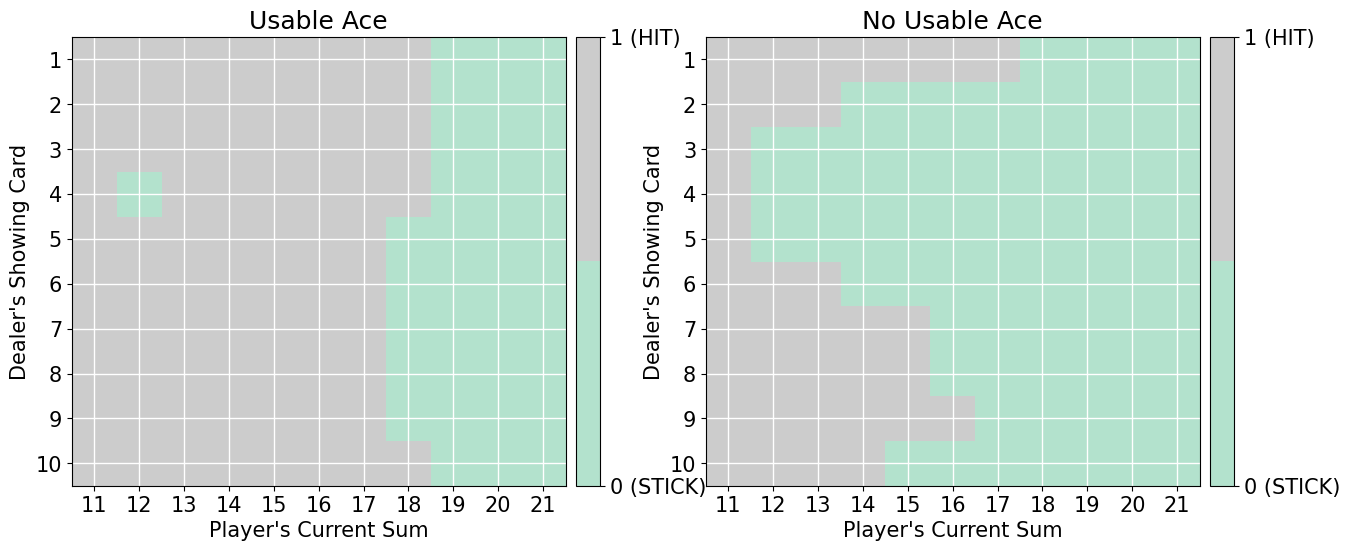
\includegraphics[width=1\textwidth]{figures/strategy.png}
\end{figure}


The learned value function is consistent with the structure of the optimal Blackjack strategy. States with higher player sums have higher value, especially when the dealer shows a weak card (2--6), since the probability of winning is high without taking additional risk. Conversely, states with low player sums have lower value, as the player is forced to hit and faces a higher risk of losing.

The presence of a usable ace significantly increases the value of a state. We also see that the value function becomes larger when the player's hand is 12, because when having a usable ace it can also be 21 (11 + 1 or 11 + 10).

The value function also reflects the dealer's strength: when the dealer shows a strong card (7--10 or ace), the value of most states decreases, as the likelihood of the dealer reaching a high total is greater. Overall, the learned value function captures the key trade-off between risk and reward and aligns well with known optimal behavior in Blackjack.

\begin{figure}[H]
    \centering
    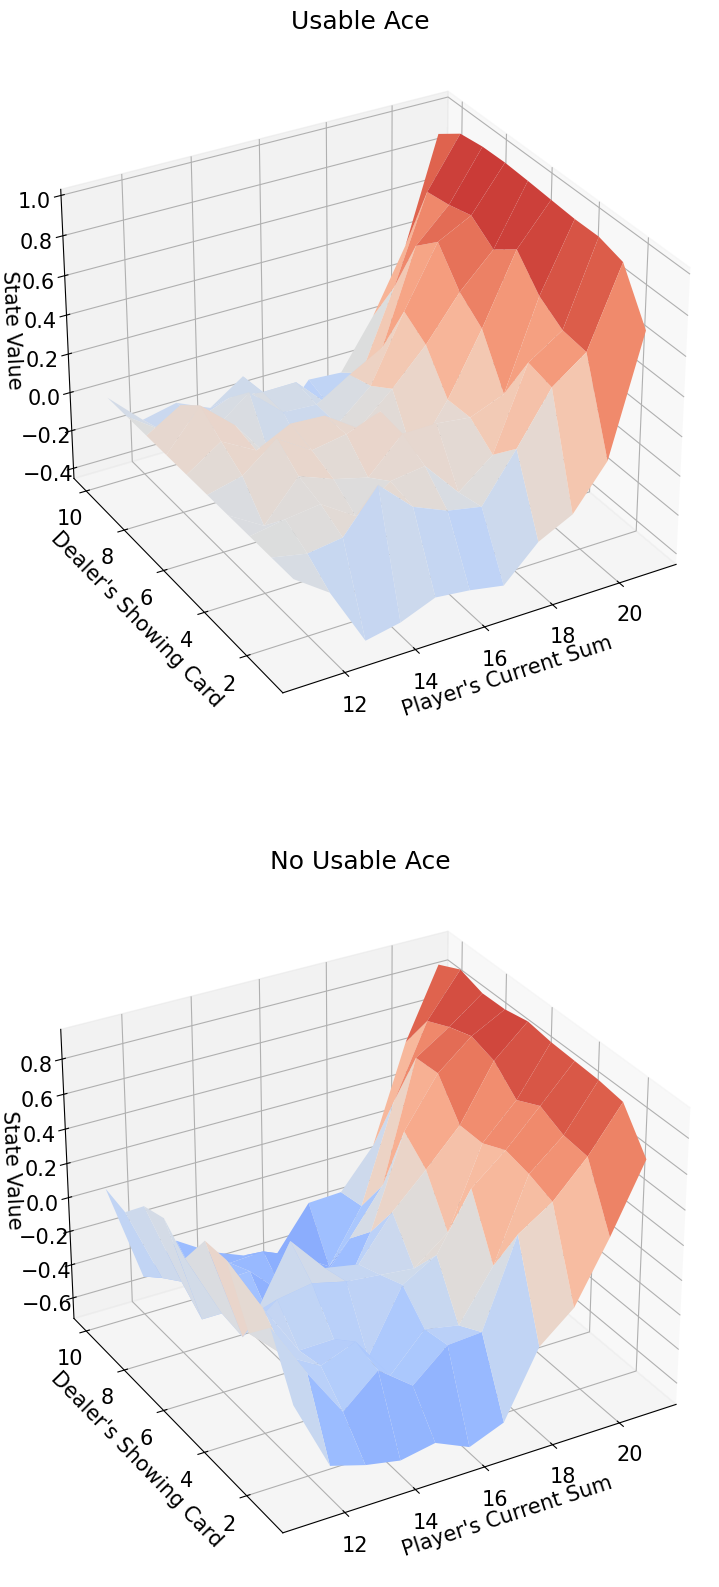
\includegraphics[width=0.6\textwidth]{figures/value_func.png}
\end{figure}


\section{Solving the Cliff World}

\subsection{Interpret the plot}

The plot shows that Expected Sarsa consistently achieves higher episode returns than Q-learning. It learns faster in the first episodes and converges to a substantially better performance level. Q-learning remains much noisier and stabilizes at lower returns.

This difference comes from the nature of the updates. Q-learning uses the maximum next-state action value, which makes it more aggressive and tends to favor the shortest path near the cliff. Because of the \(\epsilon\)-greedy exploration, this risky behavior often leads to falling off the cliff and receiving large negative rewards. Expected Sarsa instead updates using the expected value under the current policy, which better accounts for the exploratory behavior during learning. As a result, it learns a safer path that stays farther from the cliff, giving more reliable and higher returns overall.

The step-size comparison confirms this behavior. As the step-size increases, both methods improve at first, but Expected Sarsa remains consistently better over the full range. Its performance continues to improve with larger step-sizes, while Q-learning plateaus earlier and slightly degrades for the largest values. This indicates that Expected Sarsa is more stable, whereas Q-learning is more sensitive to large updates because of the variance introduced by the max operator.


\begin{figure}[h]
    \centering
    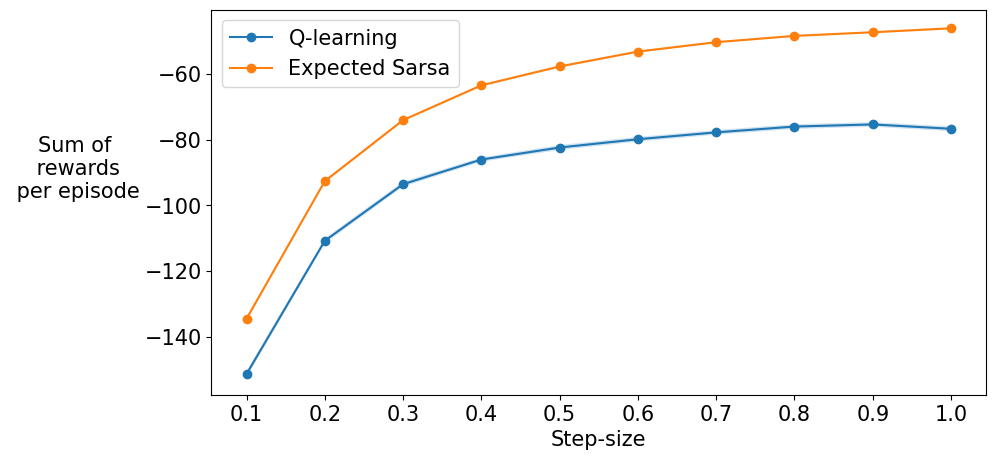
\includegraphics[width=0.48\textwidth]{figures/stepsize.png}
    \hfill
    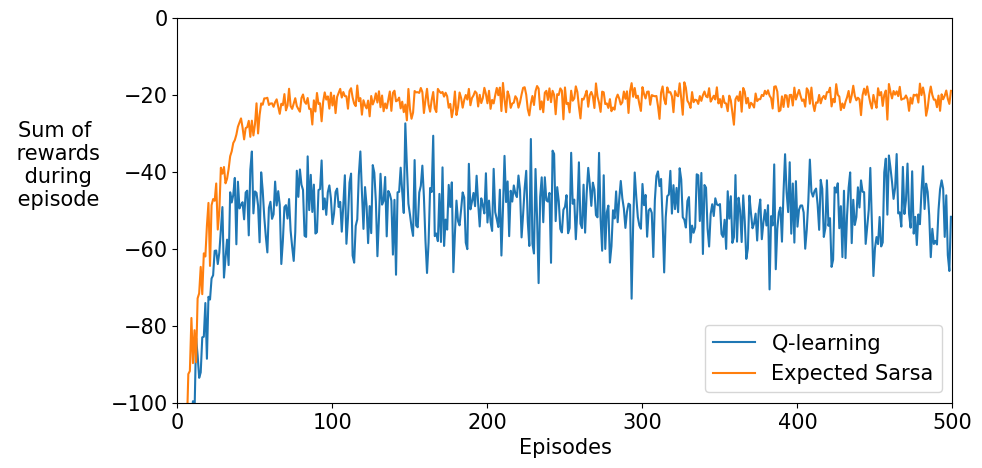
\includegraphics[width=0.48\textwidth]{figures/QVSS.png}
    \caption{Left: average return as a function of the step-size. Right: learning curves comparing Q-learning and Expected Sarsa.}
    \label{fig:cliff_results}
\end{figure}


\end{document}
